% Match the APS/PRD reprint format of paper/latex/main.tex.
% Preserve the kernel label hooks overwritten by REVTeX.
\let\OriginalLaTeXLabel\label
\documentclass[aps,prd,reprint,superscriptaddress,nofootinbib,longbibliography,floatfix]{revtex4-2}
\let\label\OriginalLaTeXLabel
\usepackage[T1]{fontenc}
\usepackage{amsmath,amssymb,bm}
\usepackage{graphicx,booktabs,xurl}
\usepackage{tikz}
\usetikzlibrary{arrows.meta,positioning}
% REVTeX's footnotes require the same microtype compatibility option as the reference.
\usepackage[nopatch=footnote]{microtype}
\usepackage[colorlinks=true,linkcolor=blue,citecolor=blue,urlcolor=blue]{hyperref}
\begin{document}

\title{Kinematic feature groups, neural network selections, and nominal
signal-strength intervals in simulated Higgs decays}
\author{[Author name]}
\email{[Corresponding-author email]}
\affiliation{[Institution and postal address]}
\date{October 29, 2026}

\begin{abstract}
We study how four kinematic input groups affect nominal signal-strength interval
widths in simulated Higgs decays to two electrons and two muons from the ATLAS
2020 educational collection. Nineteen inputs define the full ABCD representation
and four models that each omit one group. All five representations are trained
separately for seeds 42--44, using a fixed 60/20/20 allocation for training,
validation and final evaluation. Explicit four-lepton mass is excluded without
imposing mass independence. Validation-background weighted-median thresholds are
frozen before evaluation. At $10\,\mathrm{fb}^{-1}$, two score categories in one
105--140 GeV mass interval give median nominal 68\% model-self Asimov widths of
1.464392 for ABCD and 1.452977 for ABC, compared with a shared inclusive-count
width of 1.638845. Removing C widens the interval for all three seeds, while the
other ablation differences change sign. Before/after mass spectra describe the
frozen selections. All fifteen model intervals and the shared reference are
numerically valid. These completed draft001 results remain exploratory and
non-independent, with unvalidated coverage; they do not establish a calibrated
precision improvement or a physics measurement.
\end{abstract}
\maketitle

\section{Research objective and physical motivation}

The decay of a Higgs boson through two Z bosons into four charged leptons provides a setting
in which reconstructed particle kinematics can be connected to statistical inference. Near a
Higgs mass of 125 GeV, at least one Z boson is off shell. The four-lepton invariant mass
identifies the resonant region, while dilepton masses, angular relations and laboratory
momenta describe additional aspects of the selected events. These observables can help
distinguish a simulated Higgs signal from a simulated four-lepton background. Their
usefulness, however, depends on how a learning algorithm represents them and how its output
enters the subsequent analysis.

The objective of this study is to examine how physically motivated input groups affect
nominal signal-strength interval widths in a neural-network-assisted analysis. Signal
strength, denoted by \(\mu\), multiplies the expected yield of the specified Higgs signal. A
narrower nominal interval indicates tighter constraints within the assumed statistical
model. It does not establish a calibrated improvement in measurement precision. The study
therefore connects input comparisons to a defined inference procedure while examining the
physical distributions of the events selected by each network.

The comparison uses a complete input representation and four reduced
representations, each omitting one group. This design addresses the conditional usefulness
of a group when the other three remain available. It retains the feature-group research
objective while restricting the questions asked of the results. It does not search every
possible combination, assign a unique global importance to each group, or identify an
optimal compact classifier. A reduction in performance after removing a group would concern
this learner and evaluation procedure, rather than an intrinsic amount of physical
information.

A central component is the comparison of invariant-mass distributions before and after a
neural network score requirement. Signal and background are identified from their simulated
sample origins. Their yields and shapes are examined separately, so that the analysis can
distinguish overall rejection from preferential selection of particular mass regions. This
provides a physical interpretation of the learned selection alongside the interval
comparison. A more prominent signal peak is not itself evidence of a narrower or better
calibrated signal-strength interval.

The analysis uses controlled Monte Carlo (MC) samples from the ATLAS 2020 educational
collection \cite{ATLAS2020}. It includes no collision-data events and makes no claim of a
Higgs discovery, an official ATLAS or CMS result, or a physics measurement. The present
draft reports the completed simplified study and its conditional comparisons. All
numerical results below are from the new three-subset run; earlier-study numerical
results and historical template spectra are not inputs to these comparisons.

\section{Simulated samples and event definition}

The data source is the fixed pair of simulated samples already used in the project: signal
dataset identifier 345060, labelled \nolinkurl{ggH125_ZZ4lep}, and background identifier
363490, labelled \nolinkurl{llll}, from the 13 TeV collection \cite{ATLAS2020}. The signal
member defines the component scaled by \(\mu\). The background member defines the background
of this restricted study; its label alone does not establish that it is a pure
quark-initiated ZZ sample. Other Higgs production modes and additional experimental
backgrounds are outside this model. The 2020 collection is retained without mixing releases
or treating a different release as an independent validation sample.

The selected final state contains two electrons and two muons. Events must satisfy the
existing trigger, lepton identification, isolation, impact-parameter and acceptance
requirements. After these requirements, exactly four good leptons are retained and ordered
by transverse momentum. The ordered transverse-momentum thresholds are 20, 15, 10 and 7 GeV.
The event must have zero total lepton charge and valid same-flavour, opposite-sign pairs.
Electron and muon pseudorapidity acceptances remain those of the existing selection. These
requirements define a common baseline population before any network score selection is
applied.

The dilepton pair closest to the nominal Z mass is assigned to Z1, and the remaining pair
defines Z2. The existing pair-mass requirements are retained: every same-flavour
opposite-sign pair exceeds 5 GeV, with \(50<m_{Z1}<106\) GeV and \(12<m_{Z2}<115\) GeV. The
four-lepton mass is reconstructed from the summed lepton four-momenta. The analysis window
is \(105\leq m_{4\ell}<140\) GeV. Pairing, lepton ordering and angular conventions are
shared by all models; they are not changed to improve an individual classifier or a plotted
distribution.

Physical yields are normalized to an integrated luminosity of 10 fb\(^{-1}\), using the
bound sample normalization and generator weights. Negative physical weights are preserved.
Their presence does not, by itself, identify an interference contribution or justify
replacing the signed yield with an absolute-weight sum. A large simulated event sample can
still correspond to a small expected physical count after normalization and selection. The
number of stored MC events and the number of expected events in the statistical model must
therefore remain distinct throughout the interpretation.

The learning and physical-yield calculations use different measures. Training uses absolute
physical weights divided by the training-class mean absolute weight. This normalization does
not necessarily equalize the total contributions of the two classes. Validation AUC and the
threshold calculation also use absolute physical weights. Mass spectra and
inference templates instead use signed yield weights, including the appropriate sampling
normalization. Yield estimates from different data subsets refer to the same luminosity and
are not added together as separate exposures.

Repeated representations of a physical event remain together in every data assignment and
comparison. Statistical moments are formed from the total contribution of each physical
event group, rather than treating correlated rows as independent events. Invalid
reconstruction, inconsistent sample identity and unsupported physical yields are reported as
explicit failures. The study consequently compares models on the same defined population and
preserves the distinction between a physics selection, a technical failure and insufficient
simulation support.

\section{A simplified learning and evaluation procedure}

The complete representation contains nineteen inputs arranged into four groups. Table~\ref{tab:inputs}
defines both the groups and the five evaluated models. Group A describes individual leptons
in the laboratory; B describes the reconstructed dilepton systems; C describes collective
event kinematics; and D contains five decay and production angles under the existing
conventions. These groups overlap in information. A derived observable can make a
relationship easier for a finite network to learn without adding a new physical degree of
freedom. Conversely, removing an apparently useful observable can change optimization and
the resulting score partition.

\begin{table*}[tbp]
\caption{Input groups and model definitions. Part (a) specifies the retained
groups; part (b) defines the full representation and its four conditional ablations. Counts
exclude explicit four-lepton mass.}
\label{tab:inputs}
\centering
\begin{tabular}{@{}p{0.13\textwidth}p{0.72\textwidth}r@{}}
\toprule
\textbf{(a) Group} & \textbf{Inputs} & \textbf{Count} \\
\midrule
A & Four ordered lepton transverse momenta and four pseudorapidities & 8 \\
B & \nolinkurl{mZ1}, \nolinkurl{mZ2}, \nolinkurl{deltaR_Z1}, \nolinkurl{deltaR_Z2} & 4 \\
C & \nolinkurl{pt4l}, \nolinkurl{deltaPhi_ZZ} & 2 \\
D & \nolinkurl{cos_theta_star}, \nolinkurl{cos_theta_1}, \nolinkurl{cos_theta_2}, \nolinkurl{phi_decay_planes}, \nolinkurl{phi_production_plane} & 5 \\
\bottomrule
\end{tabular}


\begin{tabular}{llr}
\toprule
\textbf{(b) Model} & \textbf{Omitted group} & \textbf{Input count} \\
\midrule
ABCD & None & 19 \\
BCD & A & 11 \\
ACD & B & 15 \\
ABD & C & 17 \\
ABC & D & 14 \\
\bottomrule
\end{tabular}
\end{table*}

Explicit \(m_{4\ell}\) is excluded from all five classifiers. It is retained for the common
mass-window selection, physical diagnostics and inference definition. Excluding the mass
column does not enforce mass independence: dilepton masses, lepton momenta and other
correlated quantities can retain mass information. This study does not introduce
adversarial training, conditional score transformations or an additional mass-on comparison.
Its interpretation concerns the specified raw-score representation, including any implicit
mass dependence that survives the omission of the explicit input.

Three data subsets replace the five-role organization of the earlier procedure:
training, validation and final evaluation. All controlled MC from the two specified
members, including events in the historical test partition, enters the common
physical selection. A deterministic physical-event-group hash assigns the selected
population with probabilities 60\%, 20\% and 20\%, respectively. The
\nolinkurl{h4l-draft-v2-role-v1} assignment is common across models and training seeds
and independent of row order. These probabilities are not exact finite-sample
quotas. Table~\ref{tab:roles} states the frozen responsibilities. Final-evaluation yields use
\(w_{\rm yield}=w_{\rm physical}/0.2\), estimating the same 10~fb$^{-1}$ exposure;
subset estimates are not summed as additional luminosity.

The allocation and all fifteen models, standardization parameters, validation
thresholds and reporting rules were bound before final evaluation. An explicitly
approved access record bound to that freeze preceded evaluation. Repartitioning
previously inspected simulation does not restore independence; the run retains
its source-access history and exploratory qualification.

\begin{table}[tbp]
\caption{Frozen data responsibilities. Final evaluation begins only after
learning and threshold choices are frozen. Its use for template construction
limits the independence claims that can be made about inference validation.}
\label{tab:roles}
\centering
\begin{tabular}{@{}p{0.30\linewidth}p{0.60\linewidth}@{}}
\toprule
\textbf{Subset} & \textbf{Permitted role in this study} \\
\midrule
Training (60\%) & Fit standardization and network parameters \\
Validation (20\%) & Select the training checkpoint and determine the score threshold \\
\raggedright Final evaluation (20\%) & Apply frozen rules; construct spectra and templates; calculate nominal intervals \\
\bottomrule
\end{tabular}
\end{table}

Feature means and standard deviations are fitted on training events only and reused
unchanged for the other subsets. Each representation is trained separately; a reduced model
is not obtained by zeroing inputs of a fitted full model. The retained network has hidden
widths 64, 64 and 32, LayerNorm and SiLU activations, and dropout of 0.1 after the first two
hidden blocks. The output is a scalar sigmoid score. The score orders events under the
learning measure and is not interpreted as a calibrated physical signal probability.

Training retains AdamW with learning rate \(10^{-3}\), weight decay \(10^{-4}\), batch size
1024 and a maximum of 200 epochs. Checkpoints are selected by validation absolute-weight
AUC, with patience 20 and minimum improvement \(10^{-4}\). No architecture or hyperparameter
search is added. Input dimension changes the first-layer parameter count, so the comparison
is between representations within a common network family, not perfectly capacity-matched
learners. Three predetermined seeds, 42, 43 and 44, produce fifteen trained models. The
event split is fixed across these runs; the seeds vary training randomness rather than
generate independent data samples.

For each fitted model, the frozen threshold is the empirical absolute-weight median of
validation-background scores. Scores are ordered from low to high, and the first score whose
cumulative weight reaches at least half the total defines the threshold. Events at or above
it enter the high-score category; the others enter the low-score category. All tied scores
remain together. Ties and finite samples can produce a high-category acceptance different
from one half, and the acceptance on final evaluation need not match that on validation.
Neither effect is corrected by retuning on evaluation events.

Using validation for checkpoint and threshold selection reduces the number of data subsets
but does not make validation an unbiased final performance sample. Both choices are
completed before evaluation. Unlike the earlier joint-support selector, this procedure does
not scan a grid of cuts using evaluation-template support. If the frozen cut produces an
empty or statistically unsupported category, the candidate remains unsupported. It is not
rescued by moving the cut, changing the mass window or removing a failed seed.

Figure~\ref{fig:workflow} summarizes the sequence. Final evaluation supports an assessment of the frozen
classifier on its designated sample, subject to historical access qualifications. Because
the same evaluation events also supply the inference templates, nominal intervals
constructed from them are model-self quantities. They are not an independent test of the
likelihood's coverage or its agreement with another simulated population.

% !TeX root = main.tex
% Layout conversion of the source Mermaid graph; all ten nodes and eleven edges are retained.
\begin{figure*}[tbp]
\centering
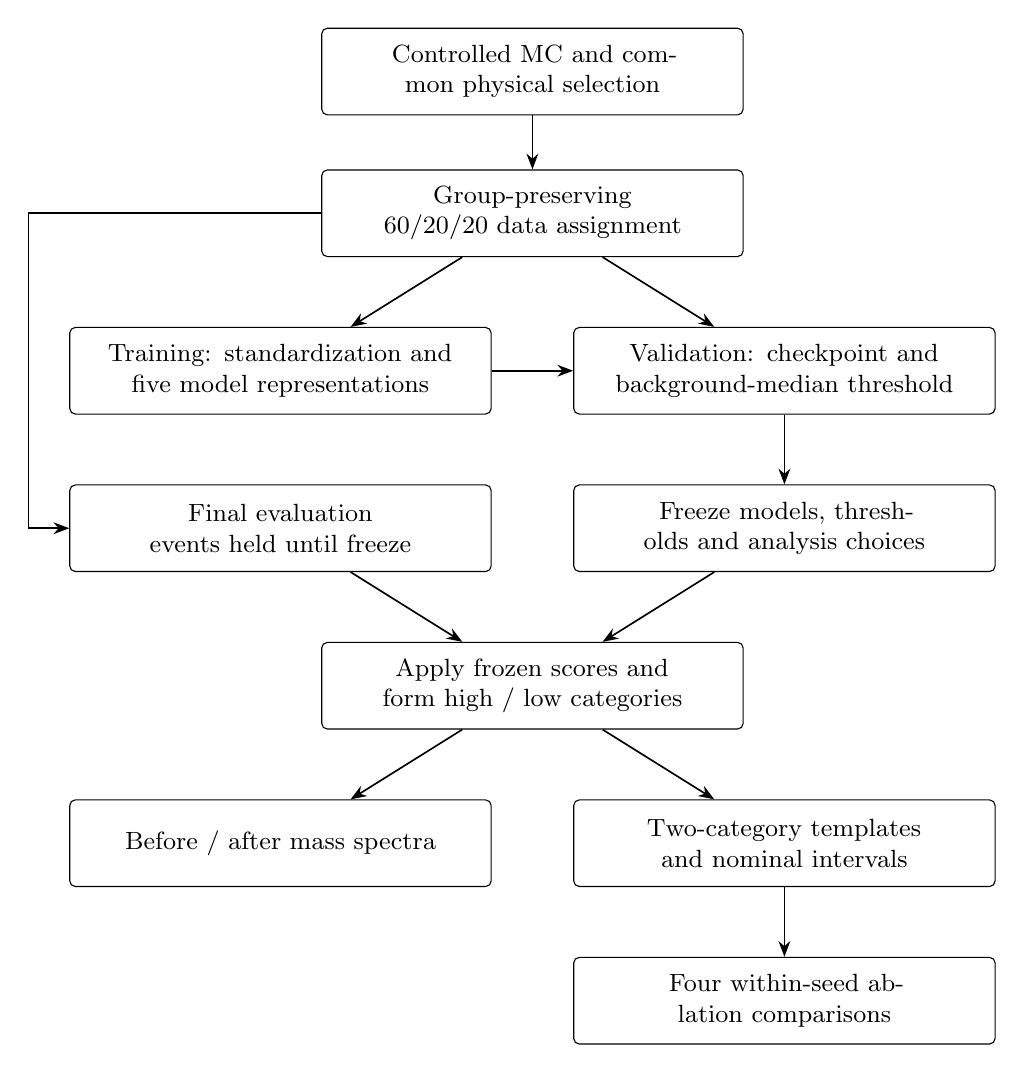
\begin{tikzpicture}[
  workflowbox/.style={draw,rounded corners=2pt,align=center,text width=5cm,
               minimum height=1.1cm,inner sep=5pt,font=\small},
  flow/.style={-{Stealth[length=2mm]},semithick}
]
\node[workflowbox] (A) at (0,0)
  {Controlled MC and common physical selection};
\node[workflowbox] (B) at (0,-1.8)
  {Group-preserving 60/20/20 data assignment};
\node[workflowbox] (C) at (-3.2,-3.8)
  {Training: standardization and five model representations};
\node[workflowbox] (D) at (3.2,-3.8)
  {Validation: checkpoint and background-median threshold};
\node[workflowbox] (E) at (3.2,-5.8)
  {Freeze models, thresholds and analysis choices};
\node[workflowbox] (F) at (-3.2,-5.8)
  {Final evaluation events held until freeze};
\node[workflowbox] (G) at (0,-7.8)
  {Apply frozen scores and form high / low categories};
\node[workflowbox] (H) at (-3.2,-9.8)
  {Before / after mass spectra};
\node[workflowbox] (I) at (3.2,-9.8)
  {Two-category templates and nominal intervals};
\node[workflowbox] (J) at (3.2,-11.8)
  {Four within-seed ablation comparisons};
\draw[flow] (A) -- (B);
\draw[flow] (B) -- (C);
\draw[flow] (B) -- (D);
\draw[flow] (C) -- (D);
\draw[flow] (D) -- (E);
\draw[flow] (B.west) -- (-6.4,-1.8) |- (F.west);
\draw[flow] (E) -- (G);
\draw[flow] (F) -- (G);
\draw[flow] (G) -- (H);
\draw[flow] (G) -- (I);
\draw[flow] (I) -- (J);
\end{tikzpicture}
\caption{Executed draft001 analysis sequence. Final evaluation followed the common
freeze and its explicitly approved access record. The high-score subset is used for the after-cut illustration; both
categories contribute to inference.}
\label{fig:workflow}
\end{figure*}



\section{Mass spectra and the physical interpretation of the selection}
\label{sec:mass-spectra}

The invariant-mass comparison addresses what the neural network selects before considering
whether its categorization changes the nominal interval. Here, ``before'' means after the
common physical baseline and mass-window requirements but before the network score cut.
``After'' means the high-score subset of that same evaluation population. Applying the cut
changes which events are retained; it does not alter the reconstructed mass of an individual
event. All comparisons use the same mass boundaries, luminosity and sample normalization.

The illustration uses the ABCD model with seed 42 and the BCD model with the same
seed, as fixed before final evaluation. BCD removes individual-lepton inputs while
retaining the other three groups. Both are applied to the same final-evaluation
population; all five models and all three seeds enter the numerical comparison.
These illustrations describe frozen selections, not independently selected
confirmation cases.

The first view uses signed physical yields. Signal and background are shown separately
before and after the cut, with consistent axes and normalization. The simulated signal is
associated with a Higgs mass near 125 GeV; its reconstructed distribution must nevertheless
be taken from the actual selected sample. The background distribution is likewise displayed
from its bound sample, rather than assigned an assumed analytic shape. This view establishes
how much signal and background survive, whether rejection is broadly distributed across the
window, and whether the selected sample becomes relatively enriched in signal.

The second view compares shapes within each process. Signal before and after selection are
normalized separately, and the analogous comparison is made for background. This separates
an overall yield reduction from a redistribution across mass. Such normalization is used
only when the signed totals and bin support permit interpretation. Negative or unstable bins
remain visible and are not clipped into an apparently smooth positive distribution. A
normalized signed histogram is not automatically a probability density.

Common 5 GeV display bins are used across 105--140 GeV. These bins are for visual
diagnostics and do not replace the single mass interval used in the inference comparison.
They can reveal broad selection dependence but cannot establish the absence of smaller-scale
distortions. For yield uncertainties, each physical event group's contribution is summed
before squaring. Before/after comparisons and normalized shapes retain the covariance
arising from shared events and shared normalization; their error bars must not be treated as
independent measurements.

The physical discussion distinguishes changes in peak visibility, overall acceptance and
distribution shape. Preferential background rejection near some masses can reshape the
continuum even without explicit mass input. A shift or narrowing of the selected signal
distribution does not demonstrate a change in detector resolution or in the physical Higgs
width. Similarly, a difference between ABCD and BCD does not uniquely identify the mechanism
used by the network. Correlations, representation convenience and training variability
remain possible explanations. The following spectra describe the new
three-subset procedure on its final-evaluation population.

% !TeX root = main.tex
% Completed draft001 final-evaluation aggregates; no event/model replay.
\subsection{Observed final-evaluation spectra}

The final-evaluation sample contains 9,049 signal and 698 background physical
event groups. The frozen validation-background thresholds are 0.746724 for ABCD
and 0.860891 for BCD at seed 42 (rounded for display). The high category uses
scores at or above the respective full-precision threshold. Both spectra use
signed yield weights divided by the 0.2 evaluation assignment probability.

The common baseline has expected signal/background yields of 2.771/2.355 at
10~fb$^{-1}$. ABCD retains 96.8\% of the signal and 51.1\% of the background;
BCD retains 94.6\% and 46.8\%, respectively. At these separately frozen cuts,
BCD rejects more of each process. These are signed-yield retentions, not the
absolute-weight acceptances used to define the validation cuts. They need not
equal the nominal 50\% validation-background acceptance.

\begin{table*}[tbp]
\caption{Signed-yield diagnostic at seed 42. Errors are grouped MC standard
errors at fixed networks and cuts. Retention errors include the shared-event
before/after covariance. Counts below are physical expectations, not MC occupancy.}
\label{tab:yields}
\centering
\begin{tabular}{llrr}
\toprule
Process & Selection & Signed yield & Retention (\%) \\
\midrule
Signal & Before & $2.7710\pm0.0293$ & --- \\
 & ABCD high & $2.6824\pm0.0288$ & $96.80\pm0.19$ \\
 & BCD high & $2.6215\pm0.0285$ & $94.60\pm0.24$ \\
Background & Before & $2.3553\pm0.1683$ & --- \\
 & ABCD high & $1.2027\pm0.1202$ & $51.06\pm3.57$ \\
 & BCD high & $1.1012\pm0.1156$ & $46.75\pm3.57$ \\
\bottomrule
\end{tabular}
\end{table*}

Figure~\ref{fig:draft001-yields} shows the simulated signal concentrated near
125~GeV. The interval $[120,130)$~GeV contains 87.9\% of its baseline signed yield,
compared with 88.6\% after the ABCD cut and 88.5\% after the BCD cut. Both selections
retain the main signal region. These coarse bins do not establish a shift in peak
position, a change in detector resolution or a change in the physical Higgs width.

\begin{figure*}[tbp]
\centering
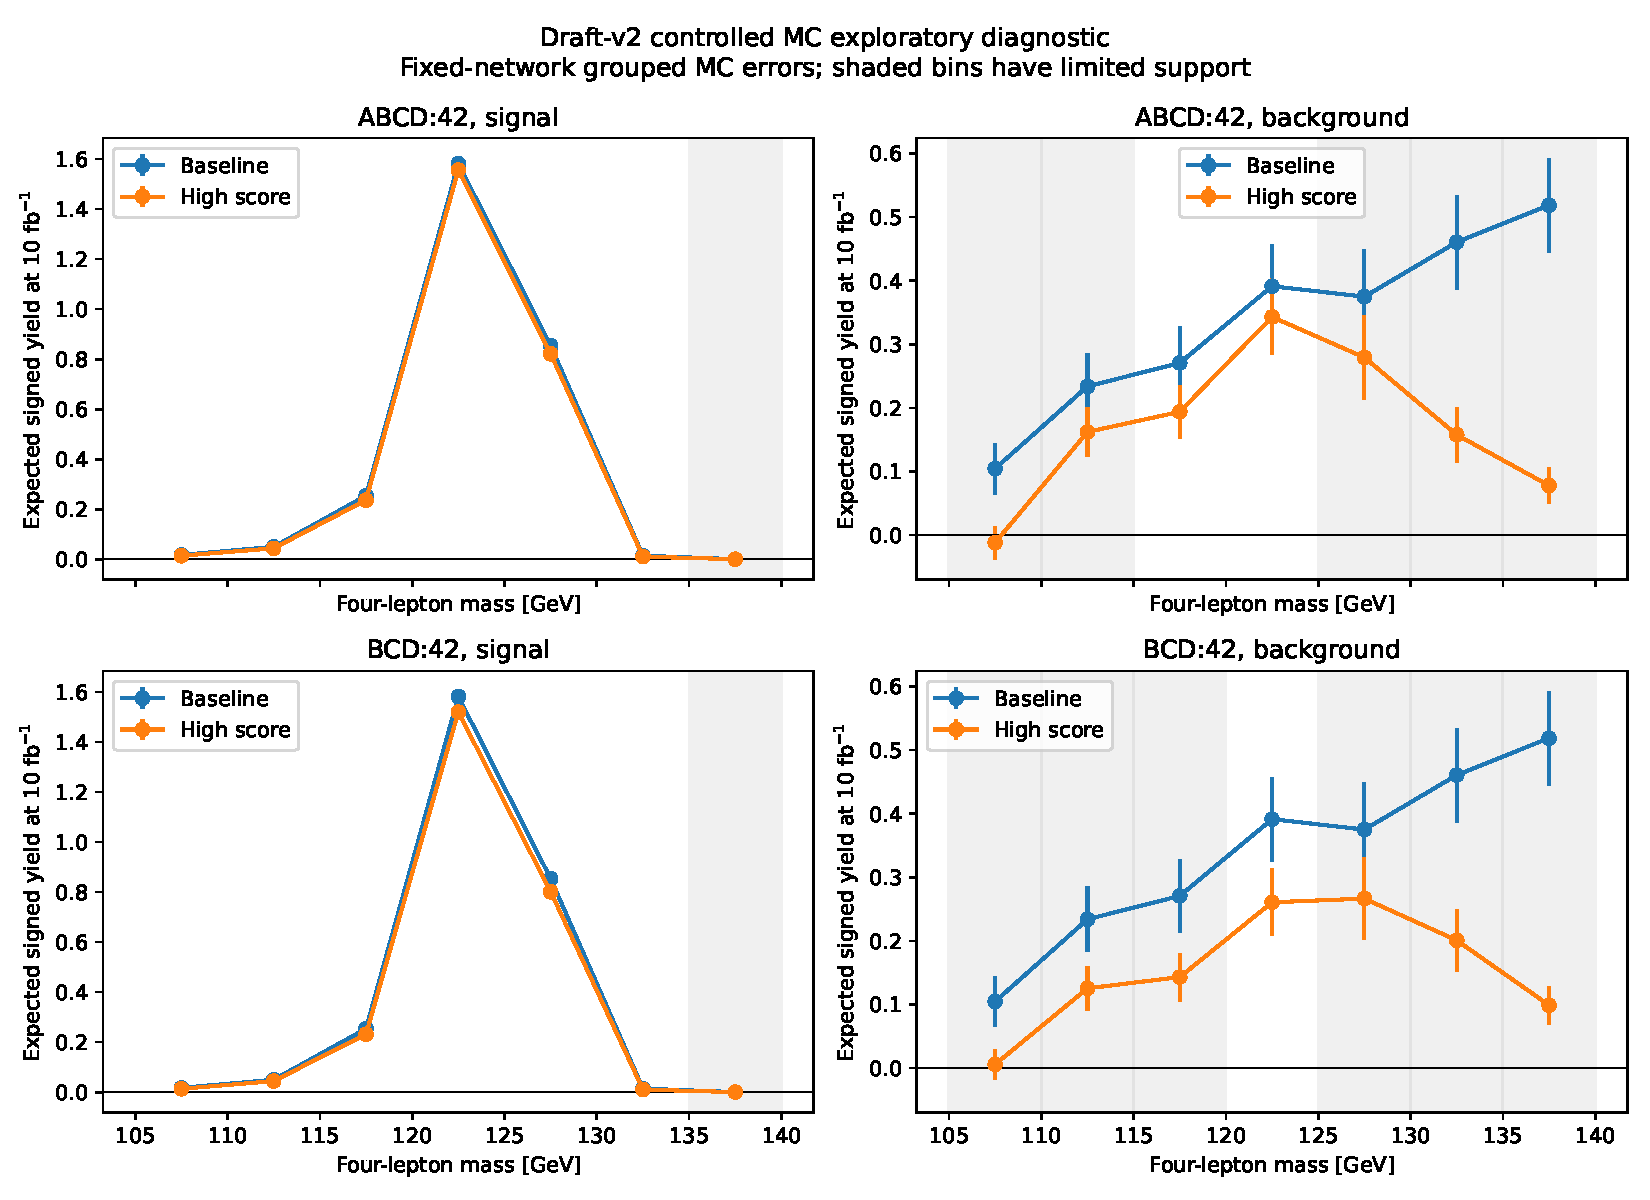
\includegraphics[width=0.88\textwidth]{figures/draft001/mass-yields.pdf}
\caption{Draft001 final-evaluation signed mass spectra at 10~fb$^{-1}$ before and
after the frozen high-score cuts. ABCD is above and BCD below, both at seed 42;
signal is left and background right. Error bars use grouped MC variance.
Shading flags low-support bins; negative yields remain visible. These seven
half-open 5~GeV display bins do not enter the likelihood, which uses one mass
interval and both score categories. Before and after curves share events.}
\label{fig:draft001-yields}
\end{figure*}

The baseline background is broad and nonuniform over the selected window. Its
signed fraction in $[120,130)$~GeV increases from 32.5\% before the cut to 51.8\%
for ABCD and 47.9\% for BCD. Its $[135,140)$~GeV fraction decreases from 22.0\% to
6.5\% and 9.0\%, respectively. Thus the selection changes background shape as well
as total yield. This is evidence of mass dependence of the frozen selections
on this MC population despite the omission of explicit mass input. It does not
identify a unique responsible feature or establish a physical background resonance.

\begin{figure*}[tbp]
\centering
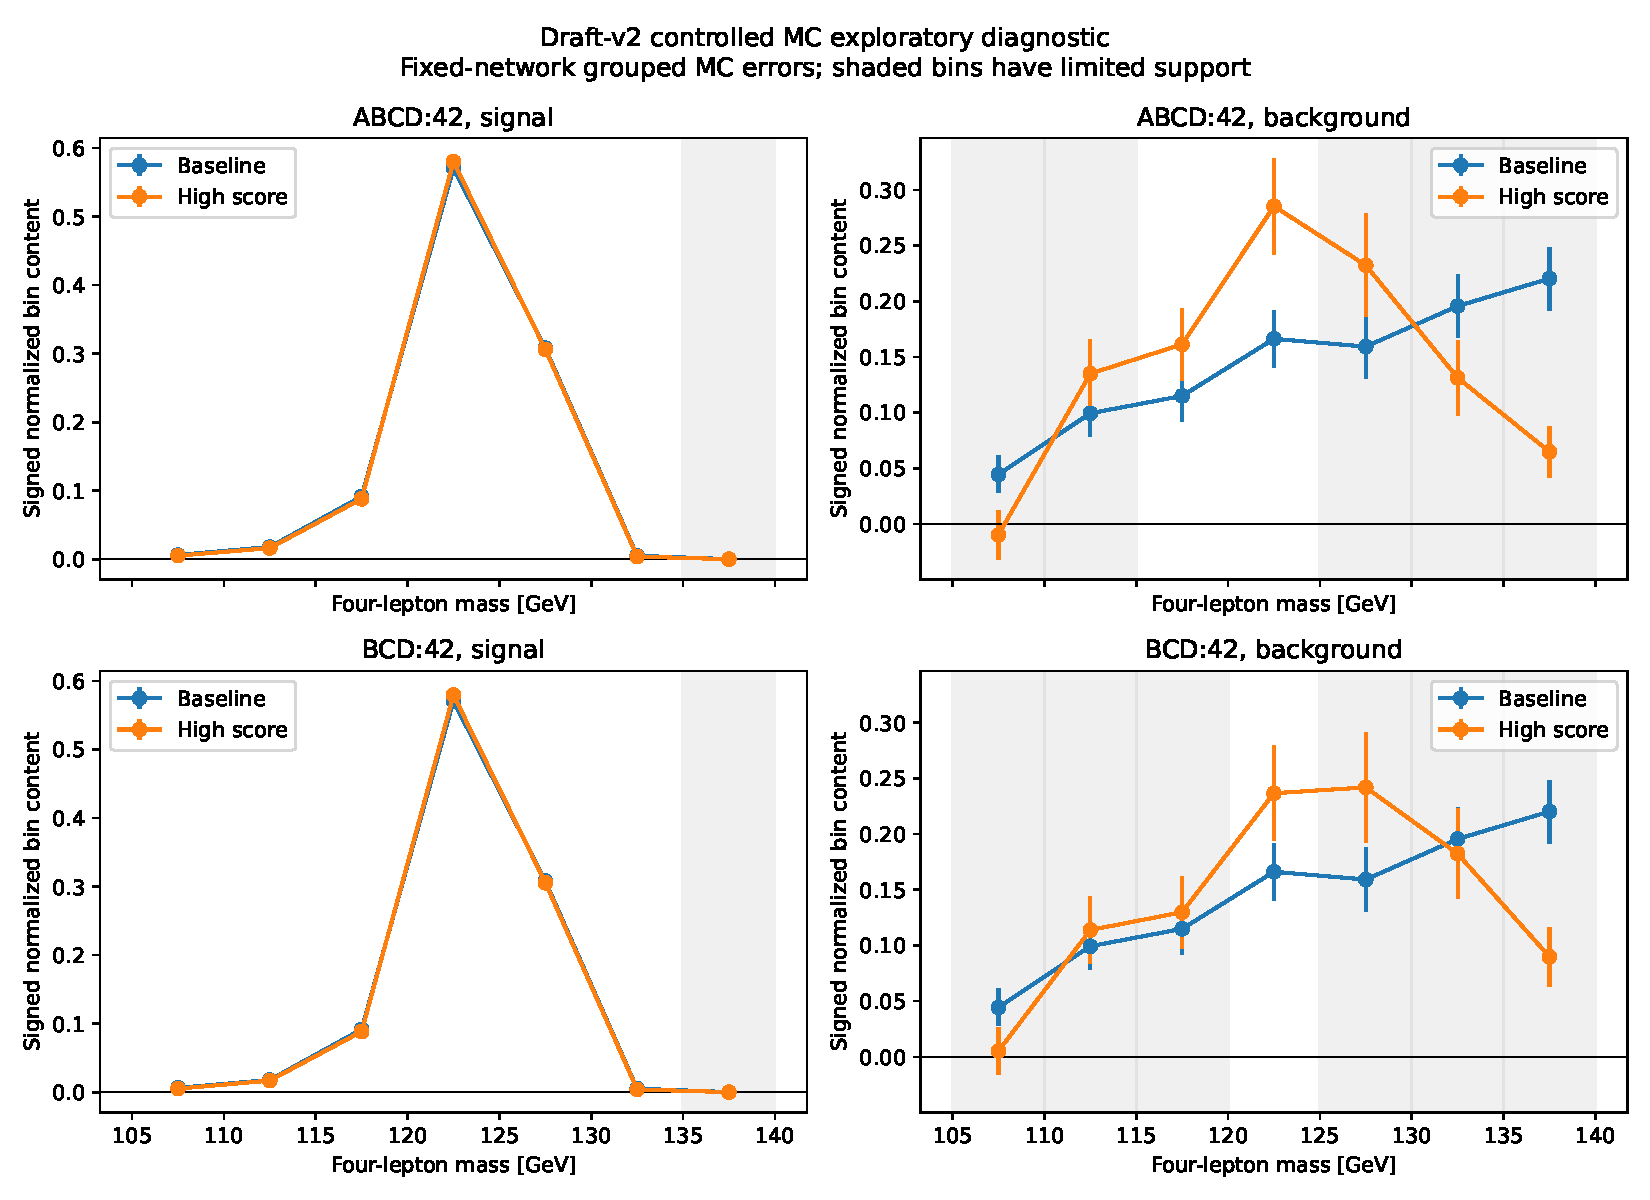
\includegraphics[width=0.88\textwidth]{figures/draft001/mass-shapes.pdf}
\caption{Draft001 before/after shapes for the same final-evaluation population
and models as Figure~\ref{fig:draft001-yields}. Each process and selection is
normalized by its own positive signed total. Errors propagate the shared
normalization; the report retains the full joint before/after shape covariance.
The error bars are therefore not independent measurements to subtract in a
shape comparison. Low-support and negative bins are retained without smoothing,
clipping or rebinning. A signed shape is not necessarily a probability density.}
\label{fig:draft001-shapes}
\end{figure*}

In particular, the selected ABCD background bin $[105,110)$~GeV has a negative
signed yield, and several background display bins have limited effective support.
The signal tail $[135,140)$~GeV also has very low occupancy. These local warnings
remain visible even though the wider mass-integrated categories satisfy the T1
support requirements. Neither the small tail differences nor the stronger visible
signal enrichment establish calibrated inference gains. All spectral errors
condition on the frozen networks and cuts; they omit threshold estimation,
independent retraining and coverage uncertainty.


\section{Nominal intervals and direct feature-group comparisons}

The primary metric remains the nominal 68\% signal-strength interval width. Each nonempty
model divides the baseline final-evaluation sample into high- and low-score categories, with one mass
interval covering 105--140 GeV in each category. Both categories enter the likelihood. Thus
the mass-spectrum illustration of the high-score subset does not mean that low-score events
are discarded from inference. The procedure compares two category counts with an
inclusive-count reference; it is not a resolved mass-peak fit.

For category \(c\), let \(s_c\) and \(b_c\) be the signed, physically normalized signal and
background expectations. At their nominal template values, the expected count is
\(\lambda_c(\mu)=\mu s_c+b_c\). The reference sums the same event population over the score
categories. It requires no trained classifier or artificial splitting of tied constant
scores. Since the population and normalization are common, its nominal result is shared
across the three training-seed comparisons. Category boundaries can vary between fitted
networks, but the inference definition remains common.

Finite simulation affects the estimates of the category yields \cite{BarlowBeeston1993}. The
retained T1 model represents this uncertainty through nonnegative multiplicative factors on
each process yield, constrained by Poisson auxiliary terms. It uses the existing pyhf
\nolinkurl{shapesys} specification \cite{pyhf2021}. The effective auxiliary count is the
squared nominal yield divided by its grouped MC variance. This is an approximation for
weighted templates, not an exact generative model for arbitrary signed samples. A successful
numerical fit does not validate that approximation independently.

Each signal/background category must have occupancy, positive signed yield and positive
variance, signed effective count of at least 20, and a cancellation ratio of at least 0.2.
The effective count compares squared yield with grouped variance; the cancellation ratio
compares the magnitude of the signed sum with the absolute-weight sum. Correlations between
category contributions from a common physical group must also be compatible with the
retained independent-category nuisance model. Unsupported rates are not replaced with
absolute values or small positive constants. These checks assess usability, not calibrated
interval coverage.

The nominal construction uses injected \(\mu=1\). For each model, the Asimov observation is
its own expected count vector, including the auxiliary expectations, without random count
fluctuations. The likelihood is profiled over the template nuisance parameters, and interval
endpoints are determined with the one-degree-of-freedom chi-squared threshold for 68\%
\cite{Cowan2011}. The physical signal-strength boundary is \(\mu\geq0\), with the retained
numerical upper search limit of 20. A missing upper crossing remains a failure rather than a
finite reported width. This construction is nominal and asymptotic; it is not a
coverage-calibrated confidence belt.

For representation \(S\) and training seed \(k\), the metric is

\[
W_{68}(S,k)=\mu_{\mathrm{upper}}(S,k)-\mu_{\mathrm{lower}}(S,k).
\]

The four primary contrasts remove one group from the full representation:

\[
\Delta W_G(k)=W_{68}(\mathrm{ABCD}\setminus G,k)-W_{68}(\mathrm{ABCD},k).
\]

A positive difference means that removing the group produces a wider nominal interval; a
negative difference means that the reduced model produces a narrower one. Neither sign alone
establishes statistical superiority or the absence of useful physics in an omitted group.
Differences are calculated within each seed before summarization. All three values and their
median are reported, rather than subtracting independently computed median widths. Shared
seed labels organize the training comparisons; shared physical event identities determine
their event-level dependence.

Table~\ref{tab:nominal} gives the complete numerical comparison: all fifteen model intervals
and the shared inclusive reference have valid numerical status. Invalid fits and unsupported categories
remain visible, and a three-seed summary is not completed by dropping an unsuccessful seed.
The median describes this small collection of trained models. Their spread measures training
variation conditional on shared MC and is not a confidence interval. Shapley values,
exhaustive interactions and a complete pairwise ranking are unnecessary for the four stated
conditional questions and are excluded from the revised analysis.

The minimal study does not include a full event-bootstrap comparison, a Toy coverage matrix
or repeated-calibration inference. Consequently, it does not quantify the complete finite-MC
uncertainty of the width differences, uncertainty from threshold estimation, or
post-selection coverage. T1 describes template uncertainty within the fitted model; it does
not supply those missing assessments. Comparisons therefore remain descriptive. Similar
widths cannot establish equivalence, and an apparently favourable median cannot establish a
confirmed precision gain.

% Source: draft001 report 9aab6d274a3e2d00d892c2d8fbf89b1e46f5b7a95d0bf0c085af90672ea36898.
\begin{table*}[tbp]
\caption{Completed draft001 nominal results. Part (a) reports all fifteen
widths; part (b) reports all twelve within-seed differences and their medians.
Values are rounded to six decimal places only for display. Every required seed
is present; no failed seed is removed. The inclusive-count reference is computed
once from the same evaluation population and has no training-seed spread.}
\label{tab:nominal}
\centering
\begin{tabular}{lrrrr}\toprule
(a) Representation & Seed 42 $W_{68}$ & Seed 43 $W_{68}$ & Seed 44 $W_{68}$ & Median \\\midrule
ABCD & 1.472197 & 1.464392 & 1.454428 & 1.464392 \\
BCD & 1.470689 & 1.474847 & 1.475575 & 1.474847 \\
ACD & 1.467509 & 1.461483 & 1.479746 & 1.467509 \\
ABD & 1.505681 & 1.513746 & 1.500712 & 1.505681 \\
ABC & 1.452977 & 1.435664 & 1.456733 & 1.452977 \\
\bottomrule\end{tabular}
\par\medskip
Shared inclusive-count $W_{68}=1.638845$ (one reference, no seed spread).\par\medskip
\centering
\begin{tabular}{lrrrr}\toprule
(b) Removed group & Seed 42 $\Delta W_G$ & Seed 43 $\Delta W_G$ & Seed 44 $\Delta W_G$ & Median $\Delta W_G$ \\\midrule
A: BCD & -0.001508 & +0.010455 & +0.021146 & +0.010455 \\
B: ACD & -0.004688 & -0.002909 & +0.025317 & -0.002909 \\
C: ABD & +0.033485 & +0.049355 & +0.046283 & +0.046283 \\
D: ABC & -0.019220 & -0.028728 & +0.002304 & -0.019220 \\
\bottomrule\end{tabular}
\par\medskip
\end{table*}


Removing C widens the interval for all three seeds, by 0.033485, 0.049355 and
0.046283, with median difference 0.046283. The differences for removing A, B or D
change sign across seeds. Their medians are respectively 0.010455, $-0.002909$
and $-0.019220$. For example, the median ACD width exceeds the median ABCD width,
but the median of their within-seed differences is negative: the paired contrast
must be formed before taking the median. These results do not establish a
universal feature ranking or statistical superiority of a reduced model.

All fifteen nominal widths are smaller than the shared inclusive-count width
of 1.638845. The full ABCD median is 1.464392 and the smallest representation
median in this five-model comparison is 1.452977 for ABC. This is a descriptive
comparison within the fixed count likelihood; it is not an uncertainty-qualified
optimization result. For scale, the ABCD seed-42 interval is
$[0.385248,1.857445]$ and the inclusive interval is $[0.298684,1.937529]$.
All sixteen lower endpoints lie above the physical boundary and all upper
crossings occur within the frozen search domain. No threshold, bin or model was
changed after final evaluation.

\section{Interpretation limits and outstanding evidence}

This simplified study can relate four conditional input changes to nominal interval widths
and to visible changes in selected event distributions. It cannot assign universal
importance to the inputs or establish that a reduced model is optimal among untested
combinations. The fixed network family, training procedure, sample composition and coarse
categorization all influence the outcome. Three seeds provide a limited check of training
stability, while the lack of independently resampled training populations limits conclusions
about generalization to other MC samples.

Physical applicability also remains restricted. The samples contain one specified Higgs
signal component and one specified background member. No untested generator, detector or
background-composition robustness is claimed. The omission of explicit mass input does not
remove implicit mass information, and the single-mass-bin inference does not measure
improvement beyond a resolved Higgs peak fit. Low expected counts, the nonnegative
signal-strength boundary and signed-template approximations constrain the interpretation of
nominal intervals even when the fitting software returns valid endpoints.

The numerical source is the completed \nolinkurl{h4l-draft-v2-draft001} run, using
its own prepared population, fifteen trained models, frozen thresholds and final
evaluation. No historical fit values or template spectra are used in Table~\ref{tab:nominal} or
Figures~\ref{fig:draft001-yields} and~\ref{fig:draft001-shapes}. The underlying
controlled MC source includes previously used events, however, and a new split or
run name cannot establish independent confirmation. The recorded qualification
remains \nolinkurl{exploratory_posthoc}, \nolinkurl{independent=false},
\nolinkurl{selection_aware_coverage=unvalidated} and
\nolinkurl{primary_claim_eligible=false}.

The 60/20/20 allocation is fixed and this run supplies its spectra, fifteen
nominal widths, shared inclusive reference, twelve paired differences and support
records. Numerical completeness does not resolve the outstanding evidence:
independent signed-MC/T1 applicability, coverage calibration, finite-MC uncertainty
of width differences, threshold-estimation uncertainty, retraining variability
across independent samples and allocation sensitivity. No bootstrap, Toy, T2,
Shapley, CDF or adversarial analysis was run for this study.

The intended contribution is a focused account of how conditional changes to the input
representation affect a specified learning and inference procedure, accompanied by a
physical explanation of the network selection. Its value depends on whether the reported
comparisons can be traced from defined simulated events through frozen scores to their
statistical interpretation. Negative, mixed or inconclusive outcomes remain valid outcomes
of that comparison. The reduced methodological scope is intended to make that chain explicit
without granting stronger scientific claims than the available evidence supports.

\begin{thebibliography}{4}

\bibitem{ATLAS2020}
ATLAS Collaboration. \emph{ATLAS 13 TeV samples collection at least four leptons (electron
or muon), for 2020 Open Data release} (2020).
\href{https://opendata.cern.ch/record/15005}{CERN Open Data record 15005}, DOI:
\href{https://doi.org/10.7483/OPENDATA.ATLAS.2Y1T.TLGL}{10.7483/OPENDATA.ATLAS.2Y1T.TLGL}.
Only the two specified simulated members are used.
\bibitem{BarlowBeeston1993}
R. Barlow and C. Beeston. \emph{Fitting using finite Monte Carlo samples}. Computer Physics
Communications \textbf{77}, 219--228 (1993). DOI:
\href{https://doi.org/10.1016/0010-4655(93)90005-W}{10.1016/0010-4655(93)90005-W}.
\bibitem{Cowan2011}
G. Cowan, K. Cranmer, E. Gross and O. Vitells. \emph{Asymptotic formulae for
likelihood-based tests of new physics}. European Physical Journal C \textbf{71}, 1554
(2011); erratum \textbf{73}, 2501 (2013). DOI:
\href{https://doi.org/10.1140/epjc/s10052-011-1554-0}{10.1140/epjc/s10052-011-1554-0}.
\bibitem{pyhf2021}
L. Heinrich, M. Feickert, G. Stark and K. Cranmer. \emph{pyhf: pure-Python implementation of
HistFactory statistical models}. Journal of Open Source Software \textbf{6}, 2823 (2021).
DOI: \href{https://doi.org/10.21105/joss.02823}{10.21105/joss.02823}. The retained model
specification is documented in the
\href{https://pyhf.readthedocs.io/en/v0.7.6/likelihood.html}{pyhf 0.7.6 likelihood
documentation}.
\end{thebibliography}

\end{document}
